\chapter{Risk factors: fruits}
\label{applications-log_normal}

Although the primary focus of the meta-regression framework developed
in this book is for estimating prevalence of disease, it is also
useful for estimating other age-specific quantities of interest in
descriptive epidemiology.  Subsequent chapters will address the
consistent estimation framework which allows data on incidence,
remission, and mortality to be included in estimates of prevalence;
this approach produces estimates of age-specific incidence, remission,
and mortality as ancillary outputs.  But before turning to that,
this chapter considers the possibility of using the
age-standardizing mixed effects spline model to produce estimates of
risk factor exposures.  An important component of the GBD 2010 Study
was the estimation of burden attributable to risk factors, and for
this chapter we focus on the descriptive epidemiology of one such
dietary risk factor, the lack of fresh fruit.

Systematic review for
risk factor epidemiology proceeds much the same as for disease
prevalence, at least for determining the population level exposure to
the risk.  In the case of lack of fruit, systematic review collected
$1502$ data points on age specific consumption of fruit, measured in
kg/day.  This is a non-negative quantity, so it is acceptable to model
with the negative binomial rate model, but it is somewhat inelegant to
do so, because this model assumes that the underlying quantity being
measured is a count, such as how many cases were observed during a
certain period of observation.  It is really the age-standardizing
mixed effects spline model that is important in risk factors
meta-regression.  In this chapter, we will compare the results of
using the negative binomial rate model with two more traditional
models for continuous data, the normal model and the log-normal model.
It turns out that, at least in this case, the differences are minimal.

Fruit consumption is a risk factor that has a significant protective
effect against morbidity and mortality from several diseases.  Fruit
consumption is measured as the total intake of fruit per day.  Fruit
includes all fresh, frozen, cooked, canned or dried fruits, excluding
fruit juices and salted or pickled fruits. \cite{he_increased_2007,
  boeing_intake_2006}

National and subnational surveys and dietary studies provided
measurement of total fruit intake via diet recalls, diet records, food
frequency questionnaires and household availability or budget surveys.
After rejecting data without measures of uncertainty, a total of $1502$
data points representing $104$ countries were included for analysis.

Often it is useful to design statistical models based on real world
processes, using count models for discrete data and rate models for
continuous data as discussed in Chapter~\ref{theory-rate_model}.
Since fruit consumption is a continuous variable, one may choose the
log normal or normal rate model over the negative binomial model to
maintain a mechanistic understanding of the statistical model.  The
models differ in their treatment of numbers that are very close to
zero, but choice of rate model does not impact the estimate,
especially with well behaved data, as seen in Figure
~\ref{fig:app-fruit rate type}.

    \begin{figure}[h]
        \begin{center}
            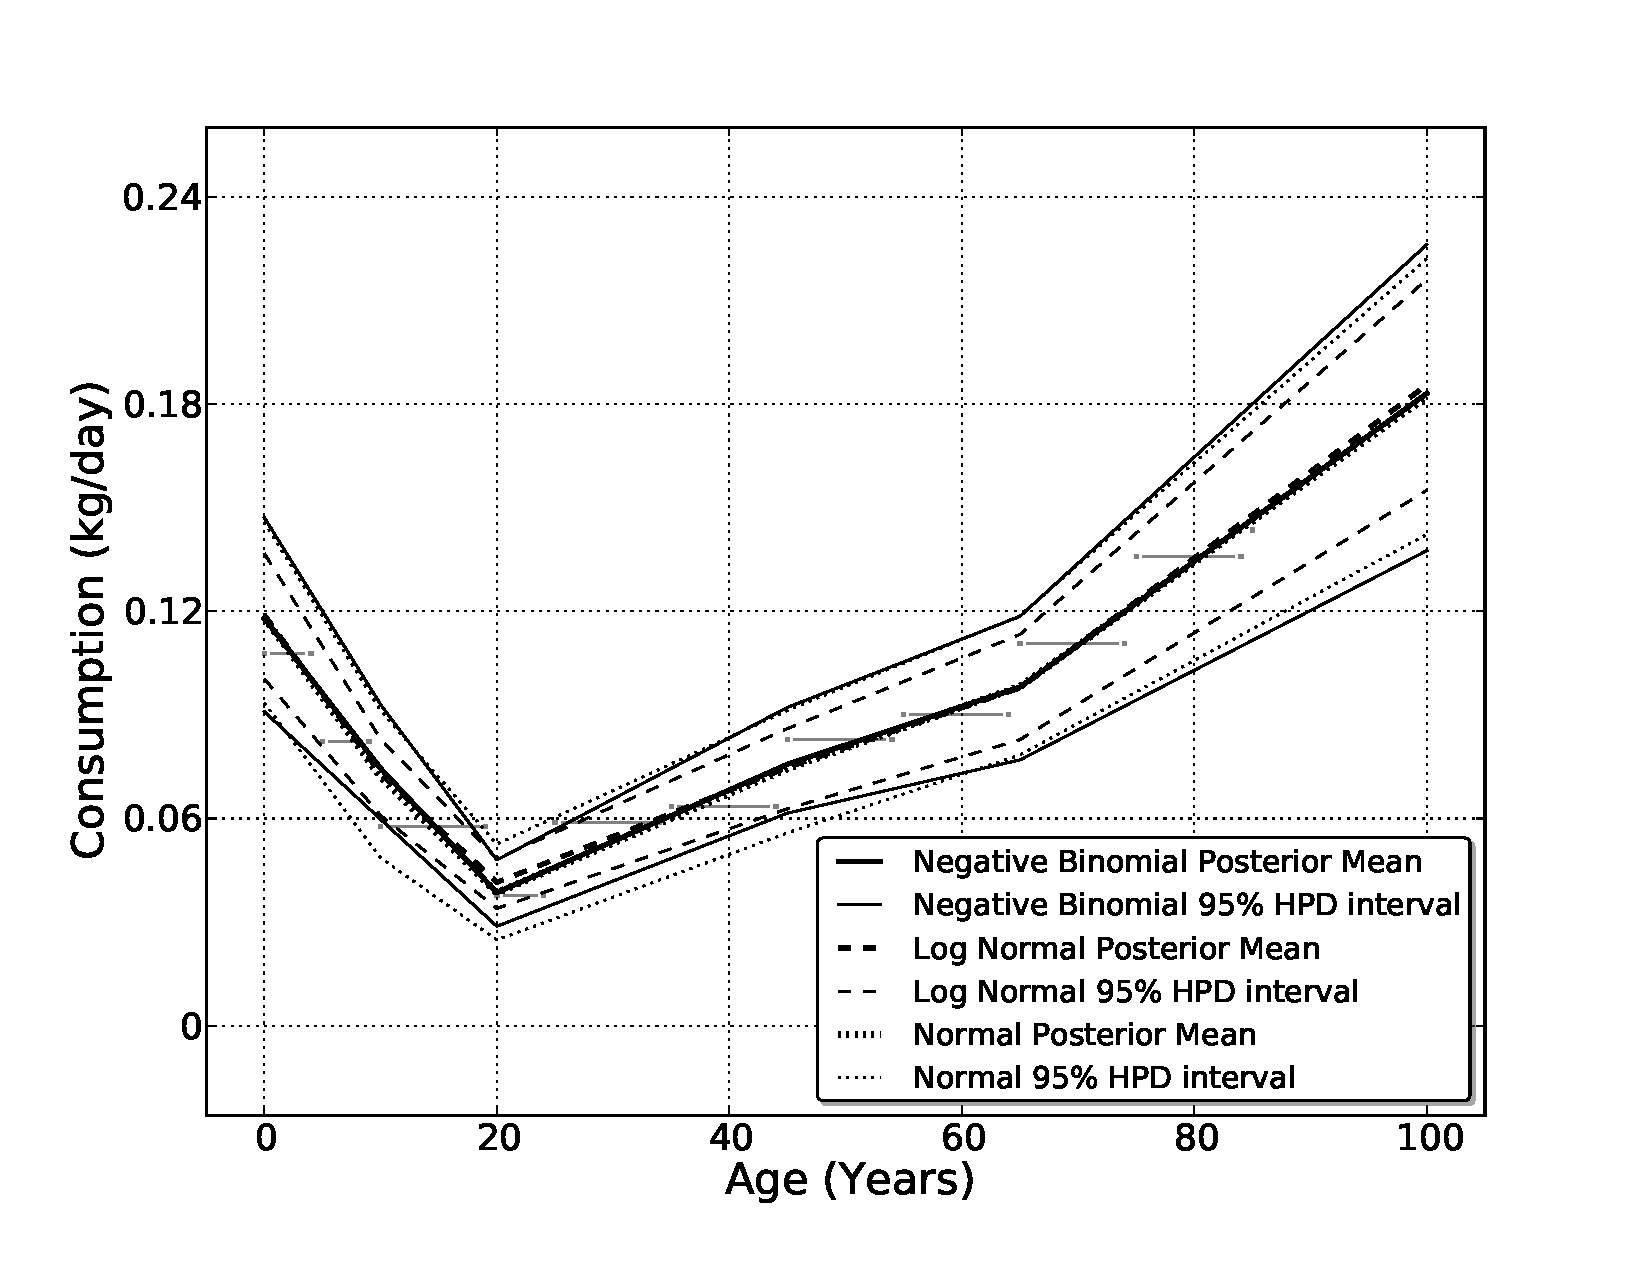
\includegraphics[width=\textwidth]{fruit-rate_type.pdf}
            \caption{Comparison of fruit consumption estimates in
              males in the United States of America in 2005 using the
              negative binomial, log normal and normal rate models.}
            \label{fig:app-fruit rate type}
        \end{center}
    \end{figure}

In an estimation setting where the data is sparser and noisier, the
models still yield quite similar results, as shown in Figure~\ref{fig:app-fruit europe},
for data from Western Europe 2005.

    \begin{figure}[h]
        \begin{center}
            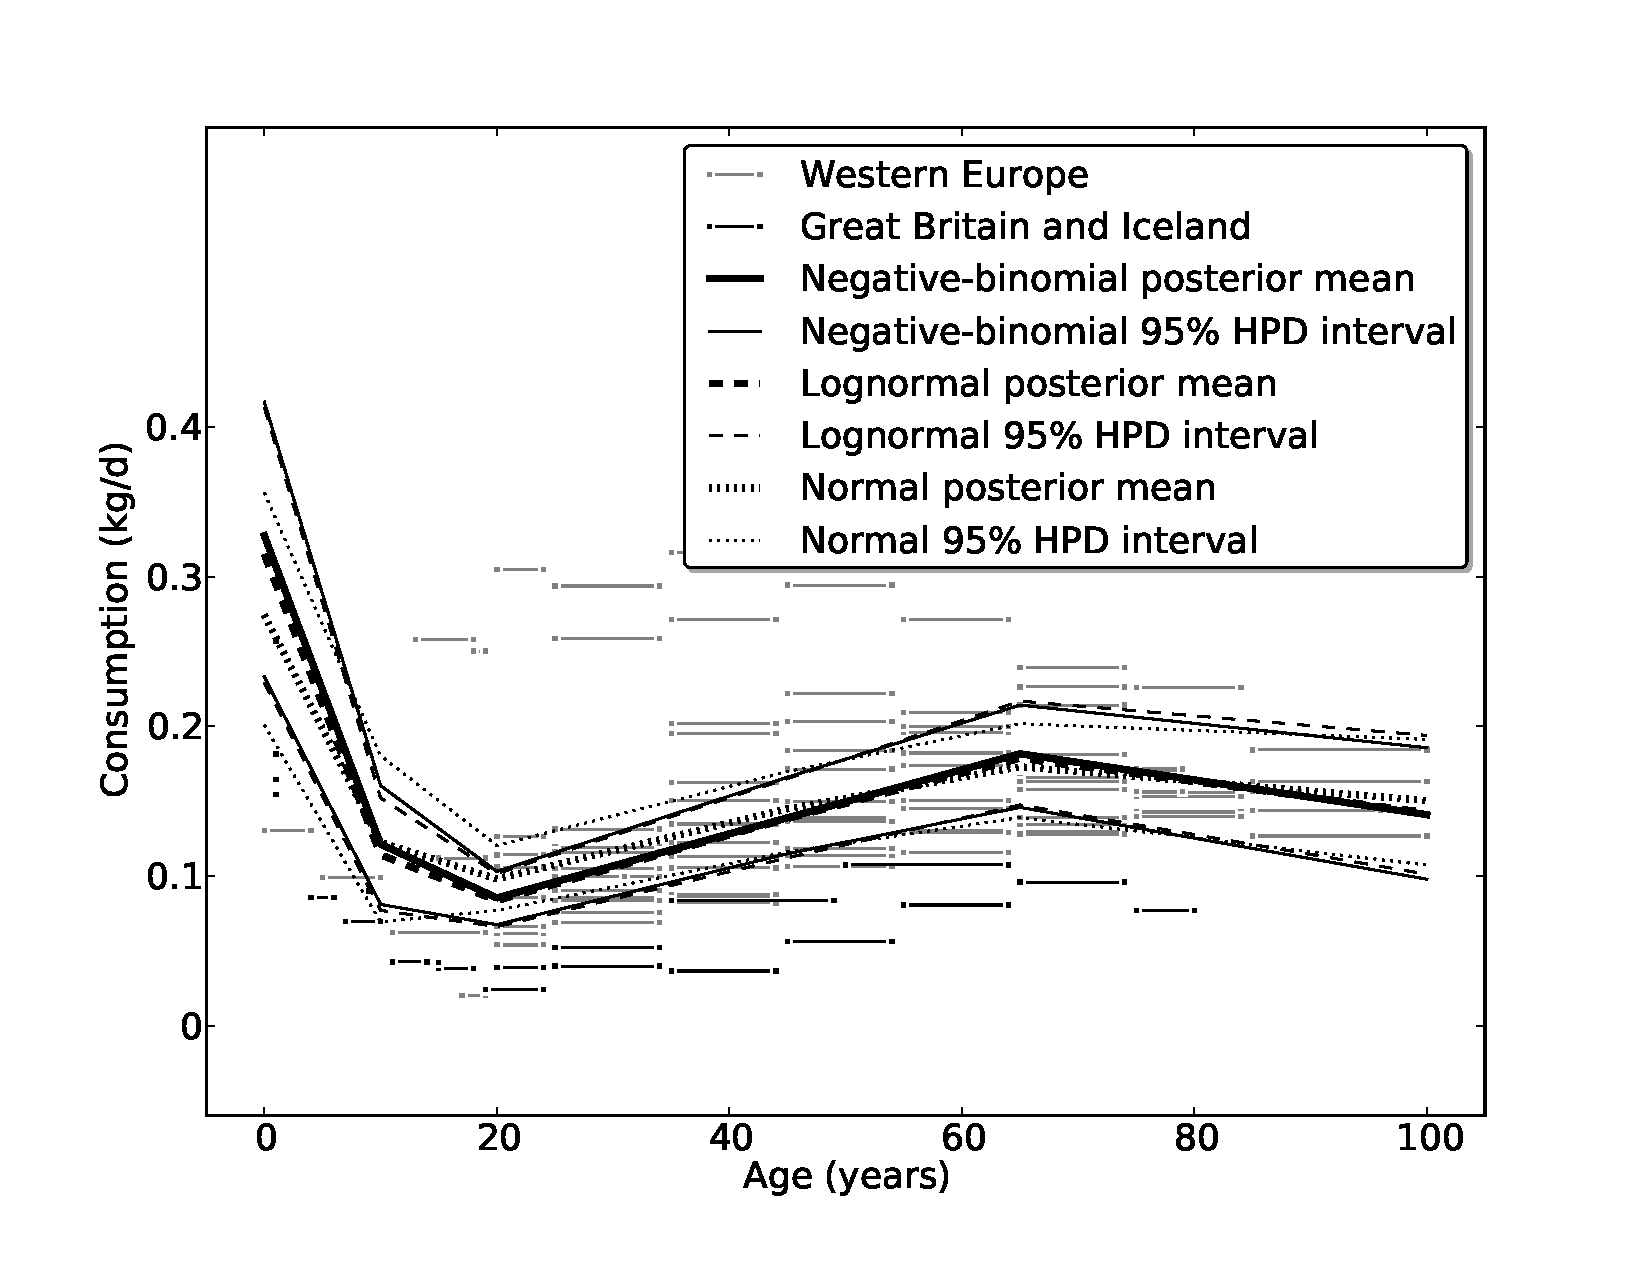
\includegraphics[width=\textwidth]{fruit-we_rate_type.pdf}
            \caption{Comparison of fruit consumption estimates in
              Western European males in 2005 using the
              negative binomial, log normal and normal rate models.}
            \label{fig:app-fruit europe}
        \end{center}
    \end{figure}

It is worth nothing that unlike the estimates in Figure~\ref{fig:app-fruit rate type}, 
Figure~\ref{fig:app-fruit europe} estimates do not go through the data at the youngest
ages (0-20).  This is because fruits have substantial country level random effects.

    \begin{table}[h]
        \begin{center}
        \begin{tabular}{|p{1.7cm}|c|c|c|}
            \hline
                & Great Britain & Iceland & Greece \\
            \hline
                negative binomial & -0.61 [-0.8, -0.4] & -0.58 [-0.8, -0.4] & 0.81 [0.7, 1] \\
                normal & -0.46 [-0.7, -0.2] & -0.41 [-0.6, -0.2] & 0.78 [0.7, 0.9] \\
                log normal & -0.88 [-1, -0.8] & -0.66 [-0.8, -0.6] & 0.67 [0.6, 0.7] \\
            \hline
        \end{tabular}
        \end{center}
        \caption{ Age-standardized Fruit consumption estimates
          from a hierarchal random effects spline model with differing
          rate models.}
        \label{tab:app-fruit rfx}
    \end{table}



